\section{Component View}
The purpose of this section is to show the component diagram which is intended to represent the internal structure of the modeled software system in terms of its main components and the relationships among them.

The following legend is used:
\begin{center}
    \begin{figure}[h!]
  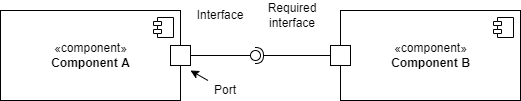
\includegraphics[width=\textwidth,height=\textheight,keepaspectratio]{./Images/ComponentLegenda.png}
  \caption{Component legend}
\end{figure}
\end{center}

All components within the diagram are described in detail below.
\begin{itemize}

\item \textbf{WebApplication}: it manages all user interactions with the web application and associates them with the required functions.

\item \textbf{MobileApplication}: it manages all user interactions with the mobile application and associates them with the required functions.

\item \textbf{AgronomistService}: This component includes the following subcomponents.

\begin{itemize}
    \item \textbf{HelpResponseService}: it allows an agronomist to manage the response to a help request received
    \item \textbf{MandalMapService}: it retrieves and displays on a mandal map relevant personal data of farmers and their performance score to the agronomist responsible of the mandal. This component is closely linked to the TableService component, which is called up as soon as the agronomist selects a farmer of interest on the map. Obviously, in order to collect all the data of interest, the component must be connected to the DatabaseAccess component. Although each farmer's location is saved in the local database, external APIs must again be used to place the farmers anywhere on the map. This is why this component is connected to GoogleMapsAPI component.
    \item \textbf{TableService}: it retrieves and displays the table of farmers’ performance in ascending order based on their performance score. Obviously, in order to collect all the data of interest, the component must be connected to the DatabaseAccess component.
    \item \textbf{DailyPlanService}: it deals with the creation and updating of the daily plan of each agronomist. Specifically, it guarantees that for each farm there are at least two visits per year by the responsible agronomist, also after changes made by the agronomist to the plan. To retrieve the scheduled plan, this component must be connected with DatabaseAccess component.
    \item \textbf{WeatherForecastsService}: it collects the data related to the weather forecasts in the mandal of a certain agronomist starting from the current day and up to the following seven days. To do this, it needs to be connected to the external API TelanganaGovernmentService as well as to the DatabaseAccess component. These data are placed on the appropriate mandal map thanks to an external API component: GoogleMapsAPI.
    \item \textbf{NotificationAgronomistService}: it deals with managing all notifications addressed to a specific agronomist, in particular whenever a help request is created in the mandal for which he/she is responsible, a notification is sent to the agronomist. In order to retrieve the notification of interest, this component is connected with the DatabaseAccess component.
\end{itemize}

\item \textbf{FarmerService}: This component includes the following subcomponents.

\begin{itemize}
    \item \textbf{HelpRequestService}: it is necessary for the creation and subsequent management of help requests by the farmer. The connection to DatabaseAccess component allows it to retrieve the recipients to whom the request can be sent (mandal agronomist and well performing farmers).\\
    In addition, if a farmer who is well performing has received a request for help from another farmer, this component takes care of managing the function that allows the farmer to respond to the request.
    \item \textbf{DiscussionForumService}: it manages the creation of posts by a farmer on the discussion forum, the creation of threads in response to a specific post (always by other farmers) and the search by topic of posts already created. It also performs these functions thanks to the connection to the DatabaseAccess component.
    \item \textbf{PerformanceService}: it takes care of updating a farmer's performance data every time he/she  enters new data about his/her crop. Not only is it necessary to connect to the DatabaseAccess, but also to external APIs to retrieve the following data: soil moisture (retrieved from CopernicusClimateDataStoreService) and quantity of water consumed (retrieved from TelanganaWaterIrrigationService).
    \item \textbf{VisitService}: it retrieve the visits that each farmer has from the agronomist in charge of his/her mandal. To retrieve them from the database, this component must be connected to the DatabaseAccess component.
    \item \textbf{WeatherConditionService}: it collects the data related to the weather conditions in the position of a certain farmer's farm for the current day. To do this, it needs to be connected to the external API TelanganaGovernmentService as well as to the DatabaseAccess component.
    \item \textbf{SuggestionsService}: it takes care of calculating the suggestions of a farmer based on his/her relevant information regarding his/her production and the position of his/her farm, data obtained thanks to the connection to the DatabaseAccess component.
    \item \textbf{NotificationFarmerService}: it deals with managing all notifications addressed to a specific farmer, in particular he/she receives notifications based on personalized suggestions, scheduled visits, help requests, replies to posts created by him/her. In order to retrieve the notification of interest, this component is connected with the DatabaseAccess component.
\end{itemize}

\item \textbf{PolicyMakerService}: This component includes the following subcomponents.

\begin{itemize}
    \item \textbf{TimeChartService}: it computes and displays Telangana’s farmers data in a graph so that the policy maker can analyze the various parameters of interest over time.
    \item \textbf{MapService}: it computes and displays Telangana’s farmers performance map using some filter. In order to collect all the data of interest, the component must be connected to the DatabaseAccess component. 
\end{itemize}

\item \textbf{AuthenticationService}: it is necessary for every type of user who wants to access the application (both from the mobile app and the web app) and use it according to the permissions he/she possesses, therefore according to the role with which he/she is registered.

\item \textbf{EmailManager}: it is necessary when a user who has not yet registered wants to register. To verify his/her email during registration, the system automatically sends a confirmation email to the user who wants to register and activates a 10-minute timer within which the user must confirm his/her registration.

\item \textbf{DatabaseAccess}: it is responsible to get data from a data source. In fact, it manages the access to the database.

\item \textbf{Database}: This component includes the following subcomponent.

\begin{itemize}
    \item \textbf{DBMS}: Database Management System refers to a software that allow users to access databases and manipulate, maintain, report, and relate data. It is used to reduce data redundancy, share data in a controlled manner, and reduce data integrity issues.
\end{itemize}

\item \textbf{ExternalAPIs}: This component includes the following subcomponents.

\begin{itemize}
    \item \textbf{GoogleMapsAPI}: it allows the connection of the application to Google Maps APIs in order to retrieve the position (latitude and longitude) of farms’ address inserted by farmers and show it on the mandal map of the agronomist. More generally, all functions that require access to geographic data not yet saved in the internal database, will rely on this component.
    \item \textbf{CopernicusClimateDataStoreService}: it is responsible for retrieving soil moisture data in the Telangana region, which is needed when a farmer wants to enter data on his/her crop. Based on the position of the farmer's farm, the system takes care of adding the soil data.
    \item \textbf{TelanganaGovernmentService}: it takes care of retrieving data relating to weather conditions relating to the position of the farmer's farm and it also has the purpose of obtaining the weather forecasts related to each mandal for which an agronomist is responsible. It also accesses ID codes' DB managed by Telangana government to check validity of ID code inserted by policy makers and agronomist while registering into DREAM. 
    \item \textbf{TelanganaWaterIrrigationService}: it is responsible for retrieving the amount of water consumed by each farmer in the Telangana region, which is needed when a farmer wants to enter data on his/her crop. Based on the position of the farmer's farm, the system takes care of adding the amount of water consumed by each farmer.
\end{itemize}

\end{itemize}

\newpage

\begin{center}
    \begin{figure}[h!]
  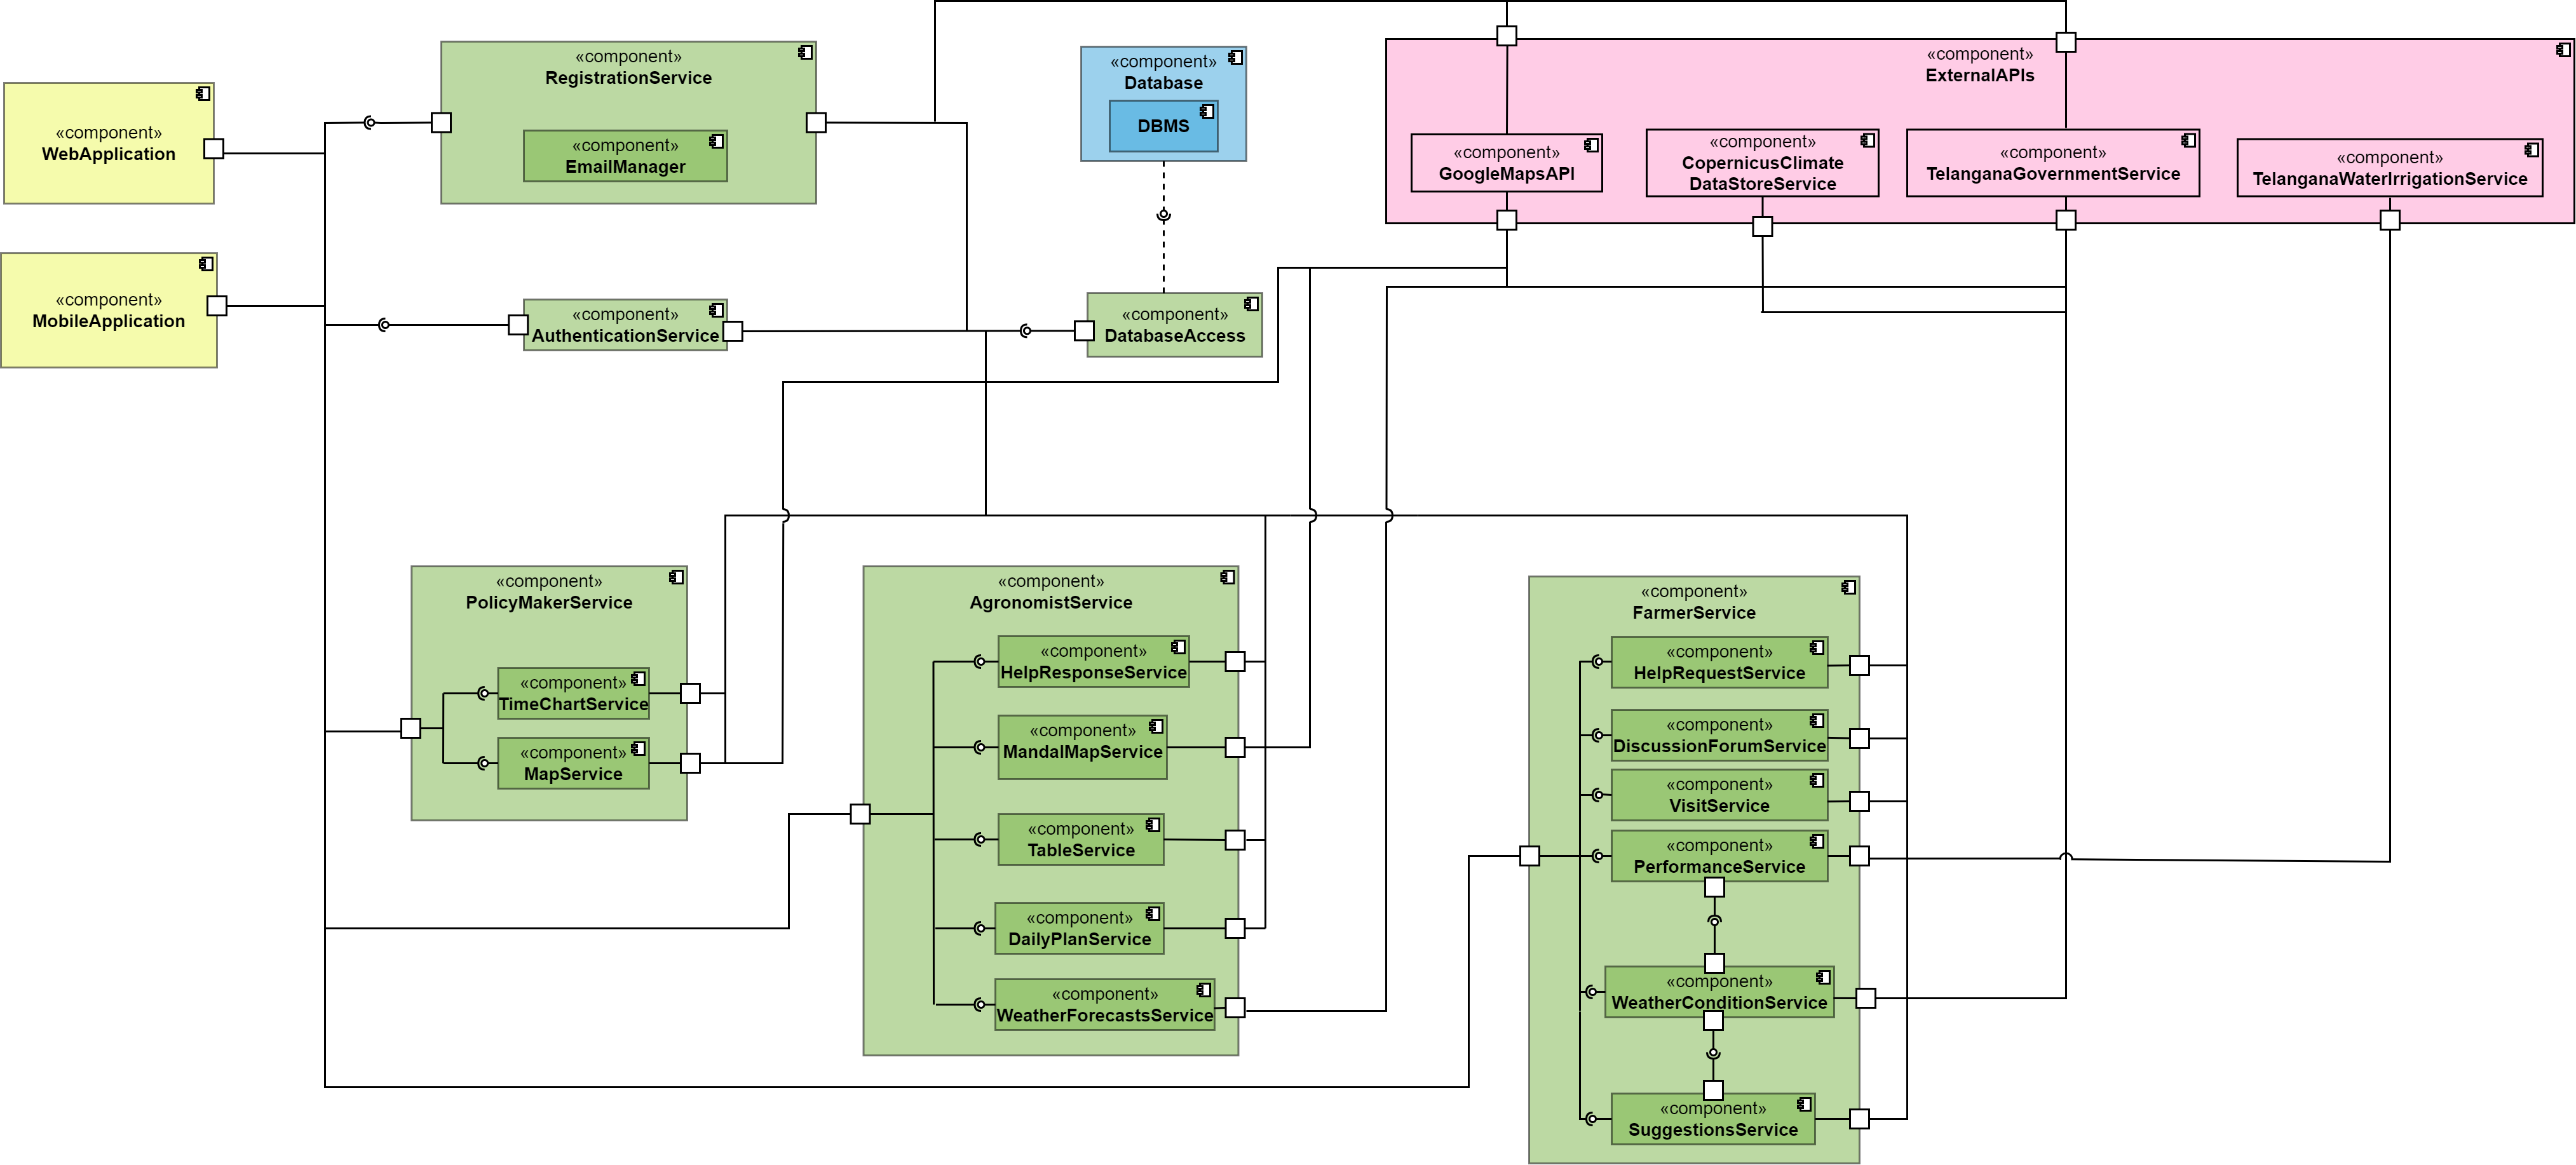
\includegraphics[width=\textwidth,height=\textheight,keepaspectratio]{./Images/Component diagram.png}
  \caption{Component diagram}
\end{figure}
\end{center}

